\documentclass[times, 10pt, twocolumn]{article}
\usepackage{latex8}
\usepackage{times}
\usepackage{url}
\usepackage{graphicx}
\usepackage{ascmac}

%\pagestyle{empty}

\begin{document}

\title{A Framework for Self-healing Device Drivers}

\author{
Hiroo Ishikawa\quad
Alexandre Courbot\quad
Tatsuo Nakajima\\
Department of Computer Science, Waseda University\\
3-4-1 Okubo, Shinjuku-ku Tokyo, Japan\\
ishikawa@dcl.info.waseda.ac.jp
}

\maketitle
\thispagestyle{empty}

\begin{abstract}
Device drivers are the major cause of operating system failure.  Prior research proposed frameworks to improve the reliability of device drivers by means of driver restart. While avoiding any instrumentation of the driver, this approach does not always allow graceful recovery. In this paper, we propose a framework for self-healing device drivers that lets the driver developer consider and implement the failure recovery of device drivers.  For this purpose, our framework provides easy to use and light-weight persistent memory that preserves the state of the driver needed to successfully recover. We developed a prototype on top of the L4 microkernel, and were able to achieve full recovery of crashed drivers as fast as 0.2 ms for different device drivers. In all cases, recovery was totally transparent for the user.
\end{abstract}


\section{Introduction}

Because of their ubiquitous and autonomous nature, embedded systems have particularly high requirements for reliability. Appliances like mobile phones and consumer electronics experience difficulty in satisfying these requirements because they get closer and closer to desktop computers as hardware evolves.  As autonomous embedded systems and their networks increasingly support our activities and lives~\cite{Lee2006}, their reliability becomes crucial in order to compensate for their lack of administration means. In particular, a failure in the system should be as much as possible hidden to the end-user.  Self-healing property to build a system that detects and repairs errors by itself has been increasing the attention of operating systems research~\cite{David2007}.  We focus on the self-healing property of device drivers, which is prone to error in operating system components.

Current embedded operating systems lack support device drivers reliability.  Prior research isolated device drivers from the operating system kernel~\cite{Herder2007,Swift2003} and handled recovery by restarting the failed driver, but this approach is not sufficient to successfully recover all classes of drivers.  Some device drivers hold important state to preserve over failure recovery,  including the current state of the managed hardware and state that is relevant across requests to the driver.  Many drivers (e.g. video, audio, webcam) change the hardware state and then wait for further requests to work with new state of the hardware.  For such drivers, a complete reset of the managed hardware is not acceptable, because (1) it has a visible side-effect for the user or other system components that would break failure transparency, and (2) future requests may lead to unexpected result on the reinitialized state.

In this paper, we present a framework for resilient device drivers that aims at solving this problem by requiring the driver to define its recovery procedure.  Since it is difficult to discriminate data that is relevant to the driver's state from neglectable data, we decided to let the programmer designate which data of the driver must be preserved across failures, using specific compiler attributes.

The framework provides persistent memory, so that not only stateless drivers, but also drivers with state such as character device drivers are able to efficiently recover in a consistent and transparent manner.  The base rule of this recovery mechanism is to only preserve what is strictly necessary to come back to the pre-failure state, and to recompute other data. Doing this, we assume that provided the bug the caused the failure is not deterministic, there is a high chance that the cause of the failure has been wiped away.

Our framework is based on the L4 microkernel architecture (commonly-used solution in contemporary embedded systems~\cite{Heiser2007}), which means that device drivers run in user mode and are isolated into protection domains, encouraging better decomposition of system services and limiting the propagation of failures to the device driver itself, an important requirement to our research.

We conducted several case studies to show the feasibility and efficiency of our device driver framework. For example, we were able to completely and transparently recover on a character device driver (parallel port driver) that failed during data transfer, without losing or duplicating any data. In addition, we were also able to recover a video driver without affecting client applications or perturbating user experience.  A fault injection test also shown that the down time of the device driver is approximately 0.2 ms.

The remainder of this paper is organized as follows.  The next section describes prior research projects on the reliability of device drivers.  Section~\ref{s:design} describes ArcOS, the operating system used to implement our work, and the idea of our framework.  Section~\ref{s:impl} details the implementation of the framework.  Section~\ref{s:eval} evaluates the framework in terms of reliability and overhead, and section~\ref{s:sum} concludes the paper.


\section{Related Work}
\label{s:rel}

Lowell et al. \cite{Lowell2000} made a classification of software failures. They distinguish between \emph{stop failures} (i.e. a program stopped because of an external reason, such as a \emph{kill} signal or a power outage) and \emph{propagation failures} (the program stopped because of an internal bug that drove it into a unacceptable state). Stop failures are easy to recover, as the interruption cause is external to the program. Therefore, provided an earlier snapshot of the running program is available, it is usually enough to restore it and pursue the execution of the program, that will this time pass the failure time successfully if the external factor that stopped it previously is not repeated again.

More challenging are propagation failures. These failures are caused by a transient bug\footnote{A transient bug or Heisen-bug is a bug that only appears occasionally and is not easily repeatable~\cite{Gray1985}.} into the running program. The time of failure and time of bug usually differ --- and can be very distant. Moreover, figuring out when the bug entered the program at the time of failure is extremely difficult. As a consequence, restoring the program to a previous state does not ensure recovery, as it is very possible that the restored state is already contaminated by the bug and will identically lead to a failure. Moreover, even if the system is restored to a state prior to the bug, nothing can ensure that the buggy conditions will not appear again during the next run.

Rx~\cite{Qin2007} tries to address this last problem by dynamically changing the execution environment based on the failure symptoms, in the hope that the change will allow the program to overtake the failure point, after which it returns to normal operation mode. Environmental changes include allocating more memory than initially asked to prevent buffers overrun, avoiding  recycle free buffers, and so on.

These recovery techniques allow to successfully recover a non-neglectable part of failure conditions. In this work, we want to address the recovery of device drivers, one class of software which is particularly exposed to transient bugs~\cite{Chou2001}, and for which failure can have very severe consequences for the whole system, as they are responsible for managing the underlying hardware.

Up to now, recovery of device drivers has been based on restarting. For instance, Nooks~\cite{Swift2003,Swift2006} isolates device drivers from the rest of the kernel and is able to transparently restart them upon failure. A similar feature is provided by MINIX 3 with its reincarnation server~\cite{Herder2007}. These recovery mechanisms are all based on the assumption that the restarted driver has no state of its own.

This is unfortunately not the case of all device drivers. For instance, character devices treat data as a stream and may fail in the middle of a transfer. In this case, simply restarting the driver and reissuing the faulty call may result in duplicated work being performed.

Another state that is important to preserve during recovery is the state of the managed hardware. Drivers typically initialize the hardware to an ``initial state'' and wait for instructions about how to control it. Such control put the hardware into a different state, and sudden reinitialization would cause a disruption in the user experience. Not to mention that applications calling the driver may still rely on the driver being in the pre-crash state, and may then issue commands that are not relevant to the reinitialized state, possibly causing the driver or the application itself to fail again.  Choices~\cite{David2007} uses transactional memory to preserve the state of operations with consistency.  However, they have performed no attempt of device driver recovery where the synchronization of software state and hardware state is necessary.

Our goal in this paper is to propose a framework for device drivers that takes recovery into account. It provides a general design pattern for drivers, as well as facilities to allow the driver maker to control recovery and restore the driver's state. In the next section, we will describe the framework's structure.

\section{A Framework For Recoverable Device Drivers}
\label{s:design}

In this section, we will describe the design of our framework for recoverable device drivers. It provides a simple way to write drivers that is consistent with the programming model of L4, and also gives the tools necessary for the programmer to consider recovery. Its recovery procedure is to restart the failed driver while preserving data that the programmer has marked as significant for the driver's consistency.

\subsection{State of Drivers Across Recovery}
\label{s:fw}

As we saw in previous section, the main issue with transient propagation failures is that they corrupt the state of the program, and invariably lead to another failure unless the corruption is cleared. Therefore, clearing the state of the failed program (e.g. through a complete restart) is the most efficient way to recover the software.  However, this extreme solution is not acceptable for all device drivers because the internal state of the driver is then completely lost.

Our strategy for recovery is to clear as much of the driver's state as possible, while preserving essential state. We restart the driver completely, but keep data that the programmer designated as significant for recovery.  Upon restart, the driver is branched to an alternate entry point that is responsible for restoring its state from this persistent data. Once  recovery is over, the driver can reprocess the request that caused its failure. Upon this restart, we expect that the faulty state has been cleared and the request reprocess will not generate the same error. If it does, this means state necessary for recovery has been corrupted, which makes transparent recovery not possible.

There are two design issues that derive from this statement:
\begin{enumerate}
\item Upon driver restart, the failing operation must be performed again.
\item The framework must be able to preserve data that is significant to the state of a driver and its managed hardware. This generally includes any internal data that cannot be recomputed identical to the pre-failure condition.
\end{enumerate}

The first requirement is easily satisfied by the design of microkernels.  In microkernels, device drivers, like any other system part, are servers that react on and reply to requests that arrive in the form of messages. By including this design into our framework, it is easy to consider a message treatment as the atomicity of our recovery system, and to send the message that triggered the failure once the driver is recovered.

As for the last requirement, the difficulty of discriminating between significant and insignificant data is what makes recovery of propagation errors difficult. If not enough state is dropped, the corruption of the system state may survive the recovery; on the other hand, if too much state is reinitialized, complete recovery is not possible and the behavior of the recovered driver may differ from its normal operation. As a recovery framework can not know what differentiates useful from futile state, we decide to let the programmer directly specify which of its variables should survive a recovery. In general however, the following rules are applied:

\paragraph{Significant state}
The state that should be preserved is classified into the following categories.
\begin{itemize}
\item Driver data that reflects the state of the hardware.  If a driver state does not reflect the state of its managed hardware, there is a high chance that the next commands issued by the driver will put the hardware into an inconsistent state.
\item Internal driver state that must survive across requests. This may include state that deals with data being provided by the managed hardware. For instance, if a character device driver sends data to the hardware from a buffer at the time of failure, recovery must be aware of the position at the time of failure in order to avoid sending the same data again.
\end{itemize}

\paragraph{Non-significant state}
This includes state that is not use to produce any side-effect and that can be recomputed by the driver, such as local data and data computed from the input message. The key of our recovery procedure is that this data is entirely reinitialized upon driver recovery, ensuring that the failure disappears provided it happened within this part of the program state.

\subsection{ArcOS}
\label{s:arc}
ArcOS is a multiserver operating system built on top of the L4 microkernel (Fig.~\ref{fig:arc})~\cite{L4X2}.  L4 provides minimum fundamental abstractions such as threads, IPC (for \emph{inter-process communication}), and address spaces. System components such as drivers run in user mode and are isolated by protection domains that are crucial for fault containment. ArcOS currently runs on the Intel IA32 architecture.

\begin{figure}[ht]
\centering
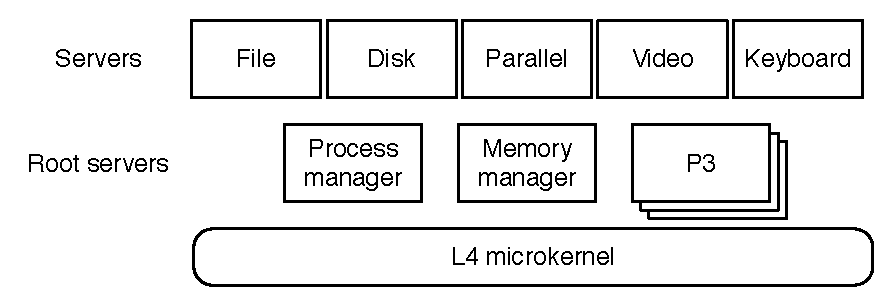
\includegraphics[scale=0.45]{figures/architecture}
\caption{Architecture of ArcOS}
\label{fig:arc}
\end{figure}

A process under ArcOS communicates with other processes via the L4 synchronous IPC mechanism. Since an IPC message payload is limited to tens of bytes, processes can use shared memory pages to exchange large amounts of data. The IPC state of a process, as well as memory page faults, are handled by its pager, a dedicated process called P3 (for \emph{Per-Process Pager}). The pager is also in charge for loading the program, which confers it a crucial role in recovery.

%\begin{figure}[ht]
%\centering
%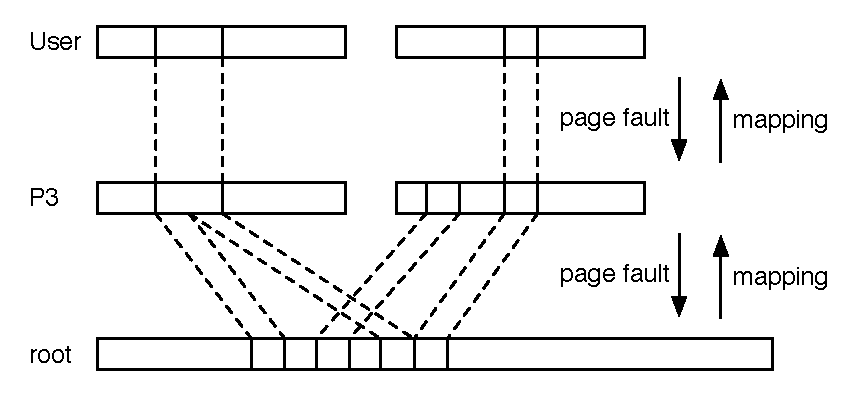
\includegraphics[scale=0.35]{figures/p3}
%\caption{The root pager, per-process pagers and user processes}
%\label{fig:p3}
%\end{figure}

This particular design, in which P3 acts as a ``nurse'' for the process it manages, increases the isolation of processes and influences how our recovery mechanism will perform.

\subsection{Driver Framework Design}
\label{sec:design-framework}
Just like any other process, a device driver is loaded and started by its own instance of P3. This particularity greatly influences the design of our driver framework. First, the task of putting the driver back into recoverable operation is left to P3. Also, the driver can have different entry points, depending on whether it is being recovered or not. We consider that there are four main states in the life of a device driver:

\begin{description}
\item[Initialization.]
Where the device driver initializes managed hardware and its internal data structures. This state is only entered once, when the driver is initially started.

\item[Service loop.]
In ArcOS, a device driver is a server process, which waits for requests from its clients: for instance, a file system server is a client of a disk driver. The service loop implements that request handling mechanism, by associating messages to handler methods.

\item[Finalization.]
In case of normal termination of the driver, this state performs operations necessary to exit cleanly, like synchronizing the hardware state to the current driver state, terminating current sessions with clients, etc. 

\item[Recovery.]
Every device driver is supposed to implement its crash recovery procedure. Should a failure occur within the driver, the framework restarts it and invokes this function instead of the initialization function. It is then up to the recovery function to ensure the driver is put back into a state where it can work again safely, by using the recovery mechanisms provided by the framework.
\end{description}

When the driver is initially started, the initialization function is called by P3, followed by the service loop and the finalization function. Should a failure occur while the driver is processing a service request, the non-persistent part of its address space is reinitialized and the driver is reloaded, entering this time the recovery function before pursuing on the service loop again (Fig.~\ref{fig:driverstatemachine}).

\begin{figure}[ht]
\centering
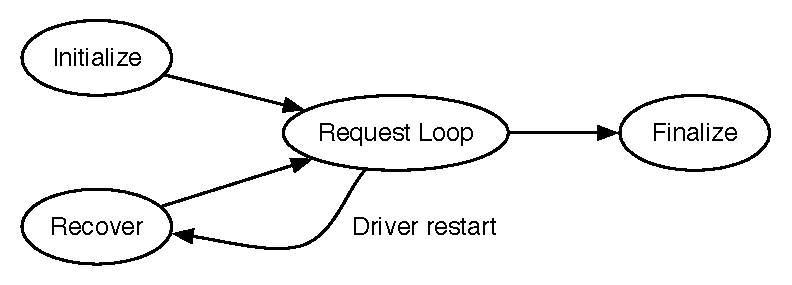
\includegraphics[scale=0.5]{figures/driverstatemachine}
\caption{States of a device driver.}
\label{fig:driverstatemachine}
\end{figure}

The framework is designed as a wrapper around the actual driver that provides this basic shape as well as other facilities for recovery (Fig.~\ref{fig:fw}). Using it, the driver writer only has to write behaviors for the initialization, finalization and recovery functions, define the protocol used by the driver to communicate with client processes, and associate function handlers to the different kinds of messages the driver can handle. Both message and error handling is then performed by the framework on this basis.

\begin{figure}[ht]
\centering
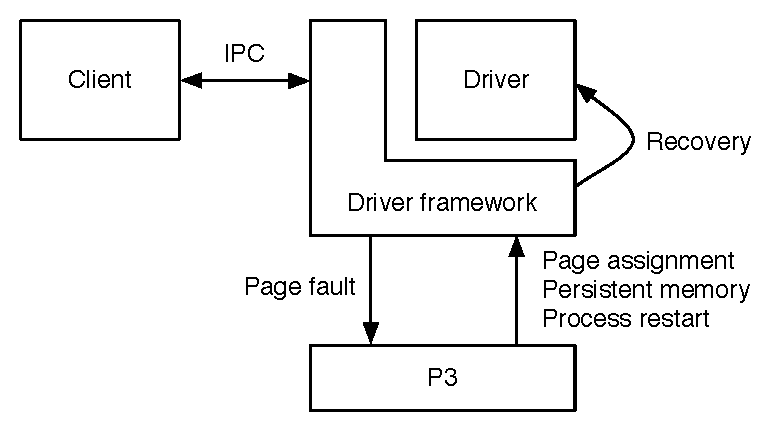
\includegraphics[scale=0.5]{figures/framework}
\caption{Device driver framework}
\label{fig:fw}
\end{figure}

Memory management and failure detection are performed by P3 which, as the driver's pager, is immediately notified of page faults and other error conditions. Should P3 detect an invalid behavior of the driver (such as a page fault to an unauthorized address, or a division by zero), it will immediately stop the driver and restart it from the recovery entry point. During the driver restart process, all its address space is cleaned and reset to its initial state, with the exception of the persistent memory area which is the only state of the driver that survives failures.


\subsubsection{Persistent memory}

When the driver fails and is restarted by P3, it tries to recover to a state that is consistent with the state of the hardware being managed so that the crash and recovery are completely transparent to other processes. Restoring to the pre-crash state requires that the data relevant to this state survives the crash. To this end, the framework provides a persistent memory area for every driver.  This area is mapped to a specific region in the driver's address space that holds data across process restart - but does not survive normal termination of the program.  Unlike a file system, the data in the persistent memory area is mapped to the physical memory so that a program deals with it as for with non-persistent data.

The framework provides a specific keyword that can be appended to variable declarations in the source code and results in these variables ending into the persistent memory area. Such declared variables remain untouched by the recovery process, and remain accessible via their pre-crash address as soon as the driver is restarted. The recovery function can thus use them to ensure the pre-crash state is recovered.

It is the responsibility of the driver writer to mark data that is relevant to recovery as persistent. Because of the variety of device drivers, there is no fixed rule to decide which data is relevant for recovery and which is not - although we listed some general guidelines in~\ref{s:fw}, each driver is unique in that respect and its author is the only qualified party to decide. This adds one extra thing to keep in mind when writing the driver, but as we will see in the experiments section the amount of code needed to ensure consistency across failures is rather light.

The set of persistent data should be as small as possible to reduce the risk of contaminating the persistent area with a propagation fault, which would result in the same failure to occur after recovery. To this end, the policy that we used during our own drivers development is to first write the driver without recovery in mind, and then make the slight adaptations that are needed to use our recovery framework. That way, variables that end in persistent memory are well-thought and chosen accordingly to the final design of the driver. We will discuss this point furthermore in the implementation and experiments sections.


\subsubsection{IPC continuation and disruption}
As every communicating process does, a device driver maintains its own IPC state.  Under our framework, in which the driver is a server replying to client requests, the state of IPC is always preserved across restart.  However, if the driver crashed before replying to the client (which is what happens unless the bug resides within the framework itself), leaving IPC state may block the client that is waiting for the reply from the driver.  To solve this problem, the framework always commit the last message it received into the persistent memory area.  When recovering, the last message is loaded from the persistent area and reprocessed. Consequently, outside processes do not notice any interruption of service.

%It shall be noted that a failed request may be processed differently in case of recovery. Requests that ask a character device driver to write or read more than one unit of data from the device may rely on a buffer and an iterator. In this case, replaying the whole request from start would result in data being written multiple times or previously read data being erased. Therefore, the handler function must be aware that the handled request is a replay of a failed previous one to behave properly. This is  possible thanks to a global status variable that is set by the framework before processing a failed request.


\subsubsection{Recovery policy}

Our recovery method is based on restart recovery.  If a driver fails, the framework restarts it to remove the cause of failure.  The framework first tries to preserve the persistent memory when restarting the driver.  If a failure still occurs despite the recovery, the framework then performs a full restart of the faulty driver--in this case, the transparency of the failure can not be guaranteed.

\section{Implementation}
\label{s:impl}

ArcOS is implemented on top of L4::Pistachio~\cite{L4X2} with experimental features. Both the framework and device drivers are implemented in C++.  By means of inheritance, the framework allows device drivers to easily implement recovery: the runtime implements common operations such as the server main loop and the definition of recovery operation flow, letting the programmer concentrate on the driver semantics.

\subsection{Driver framework}

The framework provides the \texttt{DeviceDriver} base class that enforces that all device drivers provide the mandatory operations we described in Section~\ref{sec:design-framework}. Fig.~\ref{fig:devicedriverclass} shows a simplified version of the declaration of this class.

\begin{figure}[ht]
\centering
\begin{screen}
\scriptsize{
\begin{verbatim}
class DeviceDriver {
protected:
  virtual status_t Service(
      const L4_ThreadId_t& tid,
      const L4_Msg_t& msg,
      L4_Msg_t& retMsg) = 0;
public:
  virtual status_t Initialize() = 0;
  virtual status_t Exit() = 0;
  virtual status_t Recover();
  status_t MainLoop();
};
\end{verbatim}
}
\end{screen}
\caption{Simplified version of the \texttt{DeviceDriver} class declaration.}
\label{fig:devicedriverclass}
\end{figure}

The \texttt{Initialize} and \texttt{Exit} methods are pure virtual, which enforces the driver developer to implement them. \texttt{Recover} is virtual but the framework provides a default implementation that just returns an error message to P3, stating that the driver cannot be recovered and causing a full-restart of the failed driver. Therefore, it is possible and easy to write device drivers without care about recovery.

The other public function, \texttt{MainLoop}, is already implemented and is called by P3 after the driver is started or recovered by \texttt{Initialize} or \texttt{Recover}. It waits for incoming messages, and passes them to the \texttt{Service} method along with the identifier of the sender. It also replays the failed request in case of driver recovery.

The \texttt{Service} method, although declared as pure virtual, is not to be implemented directly by the driver's writer, contrary to the other methods. This method mainly consist of a \texttt{switch} statement that checks the label of the incoming message, calls the corresponding handler, and puts the message to return to the client into \texttt{retMsg}. As it must deal with error handling and is very repetitive, we wrote a set of macros to construct it using the message/handler paradigm to associate message labels to the corresponding method handler. An example usage of these methods is given by Fig.~\ref{fig:connectors}.

\begin{figure}[ht]
\centering
\begin{screen}
\scriptsize{
\begin{verbatim}
BEGIN_HANDLERS(AudioDriver)
CONNECT_HANDLER(AUDIO_SET_VOL, SetVolume)
CONNECT_HANDLER(AUDIO_FLUSH_BUF, Flush)
...
END_HANDLERS
\end{verbatim}
}
\end{screen}
\caption{Example usage of the message/handler macros.}
\label{fig:connectors}
\end{figure}

The message labels are just integers that define the protocol used between the client and the driver and may be build using an enumeration. Handler functions must follow the following prototype:

\begin{figure}[ht]
\centering
\begin{screen}
\scriptsize{
\begin{verbatim}
status_t HandlerFunction(const L4_Msg_t& msg,
                         L4_Msg_t& retMsg);
\end{verbatim}
}
\end{screen}
\caption{Handler function prototype}
\label{fig:handler}
\end{figure}

They return the message that is to be sent back to the client in \texttt{retMsg}.

This framework provides all the necessary building blocks to write a device driver for ArcOS. By just being required to write the initialization and finalization methods and to connect messages to their corresponding handlers, the driver writer can concentrate on the functional aspect of the driver without having to worry about inter-process communication. Once the driver is written, he can then take care of the recovery aspect.

Making a driver recoverable requires to write the corresponding recovery method, and to mark relevant data to be persistent across failures.

\subsection{Persistent Memory}
The persistent memory area is designed to host data that is necessary to recovery and must therefore survive a failure. Contrary to what can be expected from a persistent memory, it does not rely on external storage and simply consists of a special part of the main memory\footnote{Real persistent storage is not necessary here as the memory must only survive driver failures, not system restart.}. Its features make it particularly suitable for embedded devices:
\begin{itemize}
\item Very lightweight: no special management is required for persistent data, which is accessed like any other data in the main memory.
\item No data redundancy: persistent data is not a duplicate of existing data, but the actual runtime data mapped to a dedicated range of the address space.
\item Easy to use: Appending a single macro to a variable declaration is enough to make it persistent.
\end{itemize}

Implementation of this persistent memory is made through a cooperation of the compiler and linker. The GCC compiler~\cite{GCCManual} provides support for section attributes that define the section of an ELF~\cite{ELFSpec} file in which a declared variable should be located. By using this feature, we defined a C macro that can be appended to any declared variable in order to place it into a special \emph{.pdata} section.

{\scriptsize{
\begin{verbatim}
#define IS_PERSISTENT \
  __attribute__ ((section(".pdata")))
\end{verbatim}
}}

At link time, the LD linker is given a special link script that relocates all data in the \emph{.pdata} section together. When P3 loads the device driver binary, it detects this \emph{.pdata} section and automatically maps it into a dedicated area of the address space.

Each process therefore possesses its own persistent memory area. P3 assigns physical memory pages to the persistent memory area at load time, just as it does with other memory sections. Upon a failure of the driver process, all the physical pages but the persistent memory area are unmapped. This design makes the persistent memory area absolutely free in terms of memory footprint, and virtually free in terms of performance, since only a few trivial operations must be performed by P3 at load and recovery time to support it.

We should note, however, that this memory is not transactional. It is not possible to bring it back to a previous state: this means that if the failure entered the persistent memory area, it will most likely not be recoverable.

\subsection{Failure Detection and Recovery}
Error detection is performed by the P3 instance of the device driver, because it is in charge of handling page faults and other kinds of exceptions. Currently we only detect memory access violation.  The error detector is implemented in the page fault handler, however, it will be improved to a general error detection architecture as proposed in~\cite{Qin2007} and~\cite{Wang2006}.

The recovery process when an invalid page access occurs (most likely due to an invalid pointer being used) is as follows: first, the faulty driver is stopped, and all its memory pages but the code and persistent data sections are unmapped. Then, the data and heap areas are reset to their initial state, and an initial stack is allocated. P3 then invokes the \texttt{Recover} method of the driver instance, which returns a status value: if that value indicates that recovery failed, P3 then fully restarts the driver from scratch. On the other hand, if the return value indicates a success, P3 sets the global recovery flag to \emph{true} and starts the driver by invoking the \texttt{MainLoop} method in the driver's address space.

The \texttt{MainLoop} method first checks the value of the global recovery flag. As its value is \emph{true}, it immediately calls the \texttt{Service} method with the last message it received before the crash. Indeed, the received message and ID of the sender are themselves placed in persistent memory, and this way IPC is not interrupted by the failure, making it completely transparent to other processes. Fig.~\ref{fig:mainloop} gives a shortened version of the \emph{MainLoop} implementation, where the error handling code has been removed.

\begin{figure}[ht]
\centering
\begin{screen}
\scriptsize{
\begin{verbatim}
static L4_ThreadId_t tid IS_PERSISTENT;
static L4_Msg_t msg IS_PERSISTENT;
status_t DeviceDriver::MainLoop() {
  status_t err;
  L4_Msg_t retMsg;
  L4_MsgTag_t tag;
  if (Recovered) goto restore;
begin:
  tag = L4_Wait(&tid);
  for (;;) {
    ...
    L4_Store(tag, &msg);
restore:
    err = Service(tid, msg, retMsg);
    ...
    L4_Load(&msg);
    tag = L4_ReplyWait(tid, &tid);
    Recovered = false;
  }
  ...
\end{verbatim}
}
\end{screen}
\caption{Shortened version of \texttt{MainLoop}.}
\label{fig:mainloop}
\end{figure}

\section{Evaluation}
\label{s:eval}

In this section, we would like to evaluate the efficiency of our driver framework. The main point for a recovery mechanism is to effectively recover upon failures. Therefore, we will illustrate how we managed to recover on two different drivers instances: first, on a character device driver (parallel port driver), a class of drivers that are particularly difficult to recover because of they handle the underlying hardware as a data stream. Then, we will consider recovering a VESA video driver. This kind of driver must keep enough information about the current state of the managed hardware to ensure a complete and transparent recovery (i.e. without graphical glitches or noticeable delay in display).

All our evaluations have been performed on an Intel Pentium4 3.4GHz with 1GB of main memory, on which ArcOS has been natively booted. We introduced failures into the drivers and observed whether they were able to recover when written without recovery in mind and when using our framework. Recovery times displayed in the performance evaluation section have been measured using L4 timers.

\subsection{Performance Evaluation}
We will first evaluate the overhead of P3.  P3 redirects all page mapping requests to the root pager, which holds the physical memory pages.  We measured the cycle count of handling a page fault and the subsequent page mapping.  Page fault handling with P3 takes approximately 1.5 times as many cycles as the one without P3.  Since page faults only occur the first time a user process accesses the page, we consider the resulting overhead as not critically harmful to performances.

Total downtime of the framework upon a failure has been measured to be 0.2 ms.  To get this metric, we injected a simple fault that results in a memory access violation, and measured the time from the fault being triggered to the {\tt Recover} method being called.  Table~\ref{tbl:recovery} shows the detail of the downtime.  The {\it Unmap} operation unmaps all the pages mapped to the driver process excepted for pages of the persistent memory.  {\it Initialize} re-initializes the counterpart of the process inside P3, which manages the base address and the size of each segment.  {\it Load} reads the binary and extracts it to the main memory. {\it Start} triggers the driver process, however, the driver doesn't immediately run because none of its pages are currently mapped.  P3 thus invokes the IPC handler which deals with page mapping requests.  According to the table, program loading takes almost half of the total time, and the remaining time is consumed by page fault handling after the driver process is restarted.

\begin{table}[ht]
\centering
\caption{Measured recovery time}
\label{tbl:recovery}
\begin{tabular}{|l|r|r|} \hline
{\bf Operation}&{\bf Time}&{\bf Rate}\\ \hline
Unmap & 28.63us & 14.33\% \\ \hline
Initialize & 0.22us & 0.11\% \\ \hline
Load & 88.46us & 44.27\% \\ \hline
Start &  8.89us & 4.45\% \\ \hline
Mapping & 73.8us & 36.9\%\\ \hline
\end{tabular}
\end{table}

To these 0.2 ms of recovery time, must be added the time necessary to invoke the \texttt{Recover} method of the driver. The execution time of this method is obviously driver-dependent. For the drivers we evaluated, the parallel driver introduces a forced latency of around 10 ms because it waits the time necessary to ensure the last written data byte (if any) has been acknowledged by the printer. The video driver, on the other hand, just requires to map the hardware framebuffer, an operation that does not take more than a couple of milliseconds.

Even when scaled to less powerful platforms such as embedded devices, we think the recovery delays will still be low enough to remain unnoticeable by the user.


\subsection{Parallel Port Driver Recovery}
Our first attempt at recovery has been performed on a very simple SPP parallel port driver. The SPP protocol is an unidirectional protocol designed to send data to a printer~\cite{Peacock2007}. Because of its simplicity, we chose to implement it in order to be able to easily demonstrate how recovery can be managed for this class of drivers.

Character devices drivers are known to be very difficult to recover; indeed, character devices deliver or receive data one unit of data at a time, and do not support random access. Therefore, if a data is read by the driver and lost in the failure, failure transparency is broken. All the same, if a service fails while sending data to a character device, transparent recovery implies that the same data is not sent twice, and thus that the driver keeps track of its internal state and uses it upon failure. Recovery solutions used in related work like Nooks~\cite{Swift2003} or MINIX 3~\cite{Herder2007} are unable to recover this class of drivers. We will show how it is possible to do it using our framework.

\subsubsection{Driver Implementation}
The driver accepts \texttt{WRITE} requests that embed the data to be written to the port. This task is performed by the \texttt{writeData} function, which writes an array of bytes to the parallel port and which simplified code can be seen on Fig.~\ref{fig:writeData}.

\begin{figure}[ht]
\centering
\begin{screen}
\scriptsize{
\begin{verbatim}
1  status_t writeData(const char *const buffer,
2                     size_t count) {
3    Byte control = inb(CONTROLPORT);
4 
5    for(int i = 0; i < count; i++) {
6      control &= ~STROBE;
7      outb(DATAPORT, buffer[i]);
8      outb(CONTROLPORT, control);
9      L4_Sleep(SEND_DELAY);
10     control |= STROBE;
11     outb(CONTROLPORT, control);
12     L4_Sleep(SEND_DELAY);
13     ...
14   }
15  ...
\end{verbatim}
}
\end{screen}
\caption{Simplified version of the \texttt{writeData} function.}
\label{fig:writeData}
\end{figure}

Writing a byte to the parallel port consists in setting the data port to the value of the byte to be written, and to lower the \texttt{STROBE} bit of the control port for at least 5 milliseconds so that the printer is aware that new data is written and readable. After that, \texttt{STROBE} is set again for 5 milliseconds before the next byte is written.

When receiving a \texttt{WRITE} request, the handler calls this function with the byte array and length of data as parameters. The rest of the driver is very simple: it has no initialization or exit function. Therefore, failures can only happen in the \texttt{WRITE} request handler and the \texttt{writeData} function, in which case P3 restarts the server and replays the last message received. If the request has not been processed at the time of failure, then recovery is completely transparent.

If the \texttt{writeData} function was in the midst of writing data from the buffer, then data may be written twice as the whole request is being reprocessed. Therefore, in order to ensure transparent recovery, we need to instrument the \texttt{writeData} function in such a way that it does not repeat already sent data.

\subsubsection{Recovery Handling}
The parallel port driver is a typical example of driver that needs to keep some intra-request data persistent in order to achieve transparent recovery. The stream nature of the parallel port also requires to keep track of the amount of processed data, symbolized by the \texttt{i} variable.

This means that \texttt{i} must be made persistent. Moreover, we have to be very careful about its time of increment: in the implementation of Fig.~\ref{fig:writeData}, \texttt{i} is only incremented at the end of the loop. If a failure occurs between the time \texttt{STROBE} is set down (line 9) and the end of the loop, the last character would be written twice when recovery takes place. Therefore, \texttt{i} must be updated right after the character is sent to the printer. Fig.~\ref{fig:writeDataRecover} gives the code of the recovery-friendly version of this method.

\begin{figure}[ht]
\centering
\begin{screen}
\scriptsize{
\begin{verbatim}
1  static int i IS_PERSISTENT = 0;
2  status_t writeData(const char *const buffer,
3                     size_t count) {
4    Byte control = inb(CONTROLPORT);
6    if (!Recovered) i = 0;
7    while (i < count) {
8      control &= ~STROBE;
9      outb(DATAPORT, buffer[i]);
10     outb(CONTROLPORT, control);
11     i++;
12     L4_Sleep(SEND_DELAY);
13     control |= STROBE;
14     outb(CONTROLPORT, control);
15     L4_Sleep(SEND_DELAY);
16     ...
17   }
18  ...
\end{verbatim}
}
\end{screen}
\caption{Recovery-friendly version of the \texttt{writeData} function.}
\label{fig:writeDataRecover}
\end{figure}

The first notable thing is that the \texttt{i} iterator is declared outside of the function to survive its local scope, and is made persistent. It is reset to zero if the IPC being processed is not the replay of a recovery\footnote{This part of the code is not really satisfactory as \textit{i} has to be explicitly reinitialized. In later versions, we plan to add several versions of the persistency macro that define the persistency scope to be either infinite, or just stand until the current request succeeds.}. Finally, \texttt{i} is incremented as soon as \texttt{STROBE} is set down, as from this time we can guarantee that the printer will receive the byte being issued if \texttt{STROBE} remains down at least 5 milliseconds.

The recovery function of the driver only has to ensure this last condition: it just waits for 5 milliseconds to ensure the current state of the \texttt{STROBE} bit is acknowledged.

\subsubsection{Results}
We tested the two versions of the parallel port driver by randomly setting the \texttt{buffer} variable and accessing it within the \texttt{writeData} function in order to make the driver fail. As expected, the non-instrumented version re-emitted the whole buffer to the parallel port, resulting in duplicated data being sent. On the other end, the recovery-friendly version never lost data, and thus recovered totally transparently.

This result is very significant regarding the capability of this framework to produce reliable drivers. Previous research on device drivers and software recovery essentially relied on simple driver restarting or resuming from a previously captured snapshot. Both methods would fail to recover this driver in most cases. Restarting the driver automatically implies that the failed IPC is entirely processed again, likely resulting in duplicate data being written. Snapshotting the entire process does not ensure that the latest snapshot is recent enough to have the data iterator up-to-date with the current state of sent data. Moreover, it is also likely that the corruption of the \texttt{buffer} variable resides in such a recent snapshot, resulting in the same failure occurring after recovery.

By letting the programmer decide which data is relevant to recovery, and by discarding all other data within the process, we ensure that important data is always preserved while maximizing chances to erase the cause of failure. This allows even very state-dependent drivers like character devices drivers to recover successfully from failures.

\subsection{VESA VBE Graphic Driver}
The VESA BIOS Extension (VBE~\cite{VBE}) specifies a standard and unified way to use graphic hardware. A program using the VBE API can use any graphic board that supports the standard.

\subsubsection{Driver Implementation}
VBE provides APIs for getting information about the video card (total memory, supported modes and their properties, etc.), setting a particular video mode, getting the hardware address of the video framebuffer, and controlling various other aspects of the graphic board. The driver that we implemented provides a view over the graphic board and its video modes to let the client programmer choose the desired video mode, as well as an access to the video framebuffer.

The video driver exposes information about the video card to the client through a shared memory page that is mapped read-only. When the client requests a video mode, the driver performs two operations: it sets the video mode to the graphic board, and maps the memory framebuffer to the client so it can draw on the screen. It also keeps the process ID of the client in memory; as the screen is not a multiplexable resource, only one program can access it at a time.

The video driver holds the following information across requests:
\begin{itemize}
\item Properties and supported modes of the video board,
\item Current holder of the screen and current video mode,
\item A mapping of the framebuffer of the current mode.
\end{itemize}

On driver failure, the first information is easily retrievable by querying the VBE API again at initialization time. However, since the driver has been restarted, this would happen in another memory page, and this duplicated information will make that the mapping of the current client would not correspond to the mapping of the driver. Also, the current holder of the screen and current video modes would be lost; which means that the driver would not know who is the current holder of the screen, or if there is even a holder. In these conditions, if another process requests access to the screen, and the driver gives it, two processes would access the screen concurrently, resulting in unpredictable results.

\subsubsection{Recovery Handling}
There are two problems to solve in order to make the VBE driver transparently recoverable. The first one is to ensure that holder and current mode information are preserved across failure. The second is to avoid querying again the video card for its capabilities and supported modes on recovery, in order to avoid wasting a memory page.

The first problem is easily solved by placing the variables for current holder and video mode into persistent memory. Since the framebuffer is recoverable from this information and its hardware address is fixed, we prefer to retrieve it again on recovery to comply with our ``preserve only the necessary'' policy.

The second problem requires that the memory page that holds card and modes information is also placed into persistent memory. As it is dynamically allocated by the driver at initialization time, this requires the use of a dedicated persistent memory allocator, which works the same way as a classical memory allocator (but on the persistent memory part of the address space). Being placed in a part of the address space that is not cleared on failure, the memory mapping of the card and mode information is preserved across failure and remain the same between the driver and its potential client.

Recovery is limited to restoring the mapping of the video framebuffer. We chose not to keep this mapping in persistent memory because it is easily retrievable, and in the case it is the source of the failure we prefer to request it again.

\subsubsection{Results}
Once the video mode is set and the framebuffer is mapped to the client process, the video driver does not interfere with the drawing operations themselves, which are directly performed by the client on the video framebuffer. It may, however, be requested for tasks like changing the beginning address of the physical screen (to support double buffering) or updating the color palette. Also, another process can request access to the screen, in which case it should be denied.

We introduced a bug in this last event that makes the driver fail, ran a graphical program, and let another process try to get access to the screen at random times. As we could expect, the recovery was effective and complete, and the graphical client not affected by the failure. Drawing operations are not conditioned by the driver being unavailable, and the only potential delays happen when the client asks the driver the change the displayed video page while the latter is being recovered, as the IPC is delayed. However, we have not perceived any visible slowdown.


\section{Conclusions and Perspectives}
\label{s:sum}

We presented a framework for writing self-healing, recoverable device drivers that is adapted to the requirements of embedded systems and should help improving their reliability. Being based on process restarting while preserving data selected by the programmer, it is very lightweight, do not involve memory-consuming operations like snapshotting, and is very fast to recover. Moreover, it is able to contain the failure and completely hide it to other processes, going as far as recovering from character devices drivers failures.

The light architecture and efficiency in recovery is obtained thanks to an active participation by the programmer who has to consider the recovery aspects of the driver by designated which data should be made persistent across failures. As we noticed by experimentation, this instrumentation is rather light (less than a dozen of lines of code to adapt on simple drivers) and the choice of data straightforward.

This recovery architecture is efficient against both stop and propagation failures. However, it becomes inefficient if the corruption that caused the failure affected data in persistent memory. Indeed, as no rollback is possible, the only chance to fix this kind of state corruption would be for the driver developer to write consistency checking and state healing code into the recovery function of the driver. Offering facilities for repairing corrupted persistent memory state, and thus increasing the failure cases that we can recover, is part of our future work.

\bibliographystyle{latex8}
\bibliography{references}

\end{document}

% vim:linebreak:
